\subsection{Calculate Radar Plot Positions}
\label{sec:ui_proc_radar_plot_pos}

This dialog allows (re-)calculation of Radar plot latitude/longitude position information based on the defined data sources and fixed field transponders (FFTs).

\begin{figure}[H]
  \center
    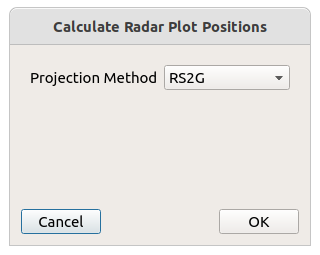
\includegraphics[width=7cm]{figures/proc_calc_radar.png}
  \caption{Calculate Radar Plot positions}
\end{figure}

Please note that for this step the Radar data source positions have to set in the database (see \nameref{sec:ui_configure_data_sources}), otherwise no plot position can be calculated.  \\

There are two projection methods (radar polar coordinates to WGS-84 coordinates) available. The \textit{RS2G} projection is the currently recommended option.

\paragraph{OGR Projection}

The EPSG code for the projection has to be chosen according to your needs, please refer to \url{http://spatialreference.org/ref/epsg/} for a list of possible codes.

The WGS84 latitude/longitude coordinates are then calculated using the radar positions in the database, the range and the azimuth. Please \textbf{note} that currently there will be offsets in the projected coordinates compared to the e.g. the ARTAS projection. The reason for this is under investigation.

\paragraph{RS2G Projection}

For this projection, no additional attributes must be given. Please \textbf{note} that this projection is based on a common 'radar slant to geodesic transformation', it should be equivalent to the ARTAS projection. A verification is still needed, please contact the author if you would be willing to support this.

\paragraph{FFTs}

The altitude of Radar plots is commonly derived from the Mode C code, and used in the slant range correction. In FFTs, the downlinked Mode C code is a configured value, often very dissimilar to the real altitude, therefore giving position errors. \\

To mitigate this unwanted behaviour, if the FFTs are correctly set in the respective configuration \nameref{sec:ui_configure_ffts}), plots generated by FFTs are identified and the FFT altitude is used for the slant range correction. The following algorithm is used for matching:

\begin{itemize}
\item Mode S Address (hexadecimal): Optional, must exist and match in plot if set in FFT, unless in CAT001
\item Mode 3/A Code (octal): Optional, must exist and match in plot if set in FFT
\item Mode C Code [ft]: Optional, must exist and match in plot if set in FFT
\item Latitude, Longitude: WGS84 position in degrees, Cartesian WGS-84 plot-FFT distance must be lower than 0.1 degrees to match
\item Altitude [ft]: Altitude above MSL, in feet, must exist and match in plot if set in FFT
\end{itemize}
\ \\

\paragraph{Usage}

Using the 'OK' button the task can be performed. During import a status indication will be shown:

\begin{figure}[H]
  \center
    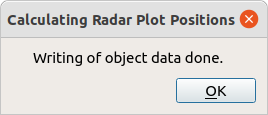
\includegraphics[width=6cm]{figures/proc_calc_radar_done.png}
  \caption{Calculate Radar Plot positions done}
\end{figure}

Please \textbf{note} that this task can be re-run with different projections if wanted.

